%%%%%%%%%%%%%%%%%%%%%%%%%%%%%%%%
% Chap 2. Background
%%%%%%%%%%%%%%%%%%%%%%%%%%%%%%%%

\chapter{Background}\label{chapter2}

%%%%%%%%%%%%%%%%%%%%%%%%%%%%%%%%
\section{Reinforcement Learning} \label{chap2:sec1}
%%%%%%%%%%%%%%%%%%%%%%%%%%%%%%%%

Reinforcement Learning (RL) is a framework in which an agent interacts with an environment and learns a policy to maximize cumulative rewards.
The agent observes the state of the environment, takes actions, and receives rewards based on those actions.
This process is formalized as a Markov Decision Process (MDP) \cite{MDP}, which provides a formal strcuture for modeling decision-making problems.
An MDP is defined by a tuple $\langle \mathcal{S}, \mathcal{A}, P, R, \gamma \rangle$, where $\mathcal{S}$ is the set of states, $\mathcal{A}$ is the set of actions, $P$ is the state transition probability function, $R$ is the reward function, and $\gamma \in [0, 1)$ is the discount factor.
In this thesis, we consider a finite-horizon setting and use the undiscounted return.
The objective of RL is to find an optimal policy $\pi^*$ that maximizes the expected cumulative reward, defined as:
\begin{equation}
  \begin{aligned}
    \theta^* &= \arg\max_\theta J(\theta) \\
    J(\theta) &= \mathbb{E}_{\tau \sim \pi_\theta} \left[\sum^T_{t = 0} r_t \right]
  \end{aligned}
\end{equation}
The policy $\pi_\theta$ is assumed to be a differentiable function parmeterized by $\theta$, denoted as $\pi_\theta(a|s)$, which represents the probability of taking ation $a$ given state $s$.
The expectation $\mathbb{E}_{\tau \sim \pi_\theta}$ is taken over the trajectories $\tau = (s_0, a_0, r_0, s_1, a_1, r_1, \ldots, s_T)$ generated by following the policy $\pi_\theta$.


\subsection{Policy Gradient Methods} \label{chap2:sec2}

Since the policy is differentiable, its gradient can be expressed using the likelihood ratio trick:
\begin{equation}
  \begin{aligned}
    \nabla_\theta \pi_\theta(s, a)
    &= \pi_\theta(s, a) \frac{\nabla_\theta \pi_\theta(s, a)}{\pi_\theta(s, a)} \\
    &= \pi_\theta(s, a) \nabla_\theta \log \pi_\theta(s, a)
  \end{aligned}
\end{equation}
This term $\nabla_\theta \log \pi_\theta(s, a)$ is referred to as the score function.
Although we previously defined the objective function $J(\pi_\theta)$ as the expected cumulative reward, we now consider a simplified case to facilitate explanation.
A one-step MDP, in which the agent takes an action from the initial state, receives a reward, and the episode terminates immediately.
Then, the objective function can be written as ($d$ is the initial state distribution):
\begin{equation}
  \begin{aligned}
    J(\theta)
    &= \mathbb{E}_{\pi_\theta}[r] \\
    &= \sum_{s \in \mathcal{S}} d(s) \sum_{a \in \mathcal{A}} \pi_\theta(s, a) R_{s ,a}
  \end{aligned}
\end{equation}
The gradient of the objective function can be computed as follows:
\begin{equation}
  \begin{aligned}
    \nabla_\theta J(\theta)
    &= \sum_{s \in \mathcal{S}} d(s) \sum_{a \in \mathcal{A}} \nabla_\theta \pi_\theta(s, a) R_{s, a} \\
    &= \sum_{s \in \mathcal{S}} d(s) \sum_{a \in \mathcal{A}} \pi_\theta(s, a) \nabla_\theta \log \pi_\theta(s, a) R_{s, a} \\
    &= \mathbb{E}_{\pi_\theta} [\nabla_\theta \log \pi_\theta(s, a) r]
  \end{aligned}
\end{equation}
The policy gradient theorem generalizes this result to multi-step MDP, where the objective function is defined as the expected cumulative reward over multiple time steps.
In other words, it replaces the instantaneous reward $r$ with the long-term value $Q^{\pi_\theta} (s, a)$, the action value function.
\begin{theorem}[Policy Gradient Theorem] \label{chap2:thm:pg}
  \begin{equation}
    \nabla_\theta J(\theta) = \mathbb{E}_{\pi_\theta} [\nabla_\theta \log \pi_\theta(s, a) Q^{\pi_\theta}(s, a)]
  \end{equation}
\end{theorem}

\subsubsection{REINFORCE}

In practice, the exact action value function $Q^{\pi_\theta} (s, a)$ is typically unknown.
Accordingly, the estimated return $G_t$ can be used as an approximation of the action value function.
In other words, the action value function $Q^{\pi_\theta} (s, a)$ can be replaced with the return $G_t$ from real sample trajectories using the Monte Carlo method.
\begin{equation}
  \nabla_\theta J(\theta) = \mathbb{E}_{\pi_\theta}[\nabla_\theta \log \pi_\theta(s, a) G_t]
\end{equation}
This leads to the Monte-Carlo policy gradient method, commonly known as REINFORCE \cite{REINFORCE}.
However, REINFORCE suffers from high variance in the gradient estimates, due to its reliance on a full trajectory.

\subsubsection{Actor-Critic}

A common approach to reducing the variance is to use a critic approximates the action value function, $Q_\phi(s, a) \approx Q^{\pi_\theta}(s, a)$.
\begin{equation}
  \nabla_\theta J(\theta) = \mathbb{E}_{\pi_\theta} [\nabla_\theta \log \pi_\theta(s, a) Q_\phi(s, a)]
\end{equation}
This is the basic idea of the Actor-Critic methods.
Actor updates the policy parameters $\theta$ and a critic updates the value function parameters $\phi$.

\subsubsection{Advantage Actor-Critic}
To further reduce the variance, we can introduce a baseline function $B(s)$.
Importantly, subtracting a baseline from the action value function does not change the gradient because its gradient is zero.
\begin{equation}
  \begin{aligned}
    \mathbb{E}_{\pi_\theta} [\nabla_\theta \log \pi_\theta(s, a) B(s)]
    &= \sum_{s \in \mathcal{S}} d(s) \sum_{a \in \mathcal{A}} \pi_\theta(s, a) \nabla_\theta \log \pi_\theta(s, a) B(s) \\
    &= \sum_{s \in \mathcal{S}} d(s) \sum_{a \in \mathcal{A}} \nabla_\theta \pi_\theta(s, a) B(s) \\
    &= \sum_{s \in \mathcal{S}} d(s) B(s) \nabla_\theta \sum_{a \in \mathcal{A}} \pi_\theta(s, a) \\
    &= 0
  \end{aligned}
\end{equation}
Therefore, subtracting a baseline function from the action value function not only leaves the gradient unchanged but also reduces its variance.
\begin{equation} \label{chap2:eq:pg_adv}
  \begin{aligned}
    A^{\pi_\theta}(s, a) &= Q^{\pi_\theta}(s, a) - V^{\pi_\theta}(s) \\
    \nabla_\theta J(\theta) &= \mathbb{E}_{\pi_\theta} [\nabla_\theta \log \pi_\theta(s, a) A^{\pi_\theta}(s, a)]
  \end{aligned}
\end{equation}
However, since the exact advantage function is generally inaccessible, both the action value function $Q^{\pi_\theta}(s, a)$ and the value function $V^{\pi_\theta}(s)$ must be approximated.
One common approach is to use the temporal difference (TD) error $\delta^{\pi_\theta}$, which is an unbiased estimator of the advantage function.
To summarize, the policy gradient has many equivalent formulations:
\begin{equation}
  \begin{aligned}
    \nabla_\theta J(\theta)
    &= \mathbb{E}_{\pi_\theta}[\nabla_\theta \log \pi_\theta(s, a) v_t] &\quad \text{REINFORCE} \\
    &= \mathbb{E}_{\pi_\theta}[\nabla_\theta \log \pi_\theta(s, a) Q_\phi(s, a)] &\quad \text{Q Actor-Critic} \\
    &= \mathbb{E}_{\pi_\theta}[\nabla_\theta \log \pi_\theta(s, a) A^{\pi_\theta}(s, a)] &\quad \text{Advantage Actor-Critic} \\
    &= \mathbb{E}_{\pi_\theta}[\nabla_\theta \log \pi_\theta(s, a) \delta^{\pi_\theta}] &\quad \text{TD Actor-Critic}
  \end{aligned}
\end{equation}

\subsubsection{Proximal Policy Optimization (PPO)}

The methods introduced above are all on-policy: training samples are collected using the same policy that we want to optimize.
However, on-policy methods can be inefficient in terms of sample usage and may suffer from instability due to large updates.
Proximal Policy Optimization (PPO) \cite{PPO} addresses these issue by incorporating importance sampling to reuse data collected from the old policy and introducing a clipped surrogate objective function to prevent large policy updates that may cause divergence.
Based on the Advantage Actor-Critic formulation Eq. \ref{chap2:eq:pg_adv}, the policy gradient can be interpreted as optimizing the following objective function:
\begin{equation}
  J(\theta) = \mathbb{E}_{\pi_\theta}[\log \pi_\theta(s, a) A^{\pi_\theta}(s, a)]
\end{equation}
This formulation assumes that data is collected from the current policy.  
However, in order to improve sample efficiency by reusing data from a previous policy $\pi_{\theta_\text{old}}$, we can apply importance sampling.
So, the objective function can be rewritten as:
\begin{equation}
  J^{\text{TRPO}}(\theta) = \mathbb{E}_{\pi_{\theta_\text{old}}} \left[ \frac{\pi_\theta (s, a)}{\pi_{\theta_\text{old}}(s, a)}A^{\pi_{\theta_\text{old}}}(s, a) \right]
\end{equation}
This objective was introduced in Trust Region Policy Optimization (TRPO) \cite{TRPO}, the predecessor of PPO.
In this formulation, $r(\theta) = \frac{\pi_\theta (s, a)}{\pi_{\theta_\text{old}}(s, a)}$ represents the probability ratio between old and new policies.
While, this allows us to reuse data from the old policy, maximizing this objective without any constraint can lead to large updates and unstable training.
To prevent such instability, PPO imposes the constraint by forcing $r(\theta)$ to stay within a small interval $[1 - \epsilon, 1 + \epsilon]$.
\begin{equation}
  J^{\text{PPO}}(\theta) = \mathbb{E}_{\pi_{\theta_\text{old}}} \left[ \min \left( r(\theta) A^{\pi_{\theta_\text{old}}}(s, a), \text{clip}(r(\theta), 1 - \epsilon, 1 + \epsilon) A^{\pi_{\theta_\text{old}}}(s, a) \right) \right]
\end{equation}
The function $\text{clip}(r(\theta), 1 - \epsilon, 1 + \epsilon)$ clips the probability ratio to the range $[1 - \epsilon, 1 + \epsilon]$.
Therefore, the objective function takes the minimum one between the original value and the clipped value.
This ensures that the policy update does not deviate too far from the old policy, thus stabilizing the training process.

%%%%%%%%%%%%%%%%%%%%%%%%%%%%%%%%
\subsection{Off-Policy Gradient Methods} \label{chap2:sec3}
%%%%%%%%%%%%%%%%%%%%%%%%%%%%%%%%

Off-policy methods allow the agent to learn from data collected by a different policy called the behavior policy.
As a result, the off-policy approach improves sample efficiency by enabling the reuse of past experiences and enhances exploration by allowing the agent to learn from data collected by a behavior policy.
In order to apply off-policy learning within the policy gradient framework, we can incorporate importance sampling into the policy gradient Theorem \ref{chap2:thm:pg}.
\begin{equation}
  \begin{aligned}
    \nabla_\theta J(\theta)
    &= \mathbb{E}_{\tau \sim \pi_\theta} [\nabla_\theta \log \pi_\theta(s, a) Q^{\pi_\theta}(s, a)] \\
    &= \mathbb{E}_{\tau \sim \beta} \left[ \frac{\pi_\theta(s, a)}{\beta(s, a)} \nabla_\theta \log \pi_\theta(s, a) Q^{\pi_\theta}(s, a) \right]
  \end{aligned}
\end{equation}
This allows to estimate the gradient using samples generated by a behavior policy $\beta$ instead of the current policy $\pi_\theta$.

\subsubsection{Soft Actor-Critic (SAC)} \label{chap2:sec3:sac}

Soft Actor-Critic (SAC) \cite{SAC1, SAC2, SAC3} is an off-policy actor-critic model.
In SAC, the policy is trained with the objective of maximizing the expected return and the entropy of the policy.
\begin{equation}
  J(\theta) = \mathbb{E}_{\tau \sim \pi_\theta} \left[ \sum^T_{t = 0} (r_t + \alpha \mathcal{H}(\pi_\theta(\cdot|s_t))) \right]
\end{equation}
\begin{equation}
  \mathcal{H}(\pi_\theta(\cdot|s_t)) = \mathbb{E}_{a_t \sim \pi_\theta}[-\log \pi_\theta(a_t|s_t)]
\end{equation}
where $\mathcal{H}(\cdot)$ is the entropy measure and $\alpha$ controls how important the entropy term is relative to the reward.
Entropy maximization leads to policies that can explore more and capture multiple modes of near-optimal strategies.
If there exist multiple options that seem equally good, the policy should assign each of them an equal probability.
In the SAC algorithm, the policy is updated through the soft policy iteration.
First, the policy evaluation step of soft policy iteration computes the soft Q-value:
\begin{equation}
  Q^{\pi_\theta}(s, a) = \mathbb{E}_{\tau \sim \pi_\theta} \left[ \sum^T_{t = 0} \left(r_t + \alpha \mathcal{H}(\pi_\theta(\cdot|s_t))\right) \Big| s_0 = s, a_0 = a \right]
\end{equation}
Then, the policy improvement step updates the policy to minimize the KL-divergence:
\begin{equation}
  \begin{aligned}
    J(\theta)
    &= \mathbb{E}_{s_t \sim \mathcal{D}} \left[ D_\text{KL} \left( \pi_\theta(\cdot|s_t) \Big|\Big| \frac{\exp(Q_\theta(s_t, \cdot))}{z_\theta(s_t)} \right) \right] \\
    &= \mathbb{E}_{s_t \sim \mathcal{D}} \left[ \mathbb{E}_{a_t \sim \pi_\theta} [\alpha \log (\pi_\theta(a_t|s_t)) - Q_\phi(s_t, a_t)] \right]
  \end{aligned}
\end{equation}

%%%%%%%%%%%%%%%%%%%%%%%%%%%%%%%%
\section{Constrained Reinforcement Learning} \label{chap2:sec4}
%%%%%%%%%%%%%%%%%%%%%%%%%%%%%%%%

Constrained Reinforcement Learning (CRL) extends the standard RL framework by incorporating constraints into the learning process.
CRL is formalized as a Constrained Markov Decision Process (CMDP) \cite{CMDP}, which is defined by a tuple $\langle \mathcal{S}, \mathcal{A}, \mathcal{P}, \mathcal{R}, \mathcal{C}, \gamma \rangle$.
Here, $\mathcal{C}$ is the cost functions associated with the constraints.
The feasible policy set in a CMDP is given by:
\begin{equation}
  \Pi_C = \{\pi: J_{c_i}(\pi) \leq d_i, \quad i = 1, \cdots, k\}
\end{equation}
where $J_{c_i}(\pi)$ is a cost-based constraint function defined the expected cumulative cost, and $d_i$ is the threshold for the $i$-th constraint.
The objective of CRL is to find an optimal policy that maximizes the expected cumulative reward while satisfying the constraints.
In the context of policy gradient methods, the constrained optimization problem can be formulated as follows:
\begin{equation} \label{chap2:eq:crl-objective}
  \begin{aligned}
    \theta^* &= \arg\max_\theta J(\theta) \\
    J(\theta) &= \mathbb{E}_{\tau \sim \pi_\theta} \left[ \sum^T_{t = 0} r_t \right] \; \text{subject to} \; \mathbb{E}_{\tau \sim \pi_\theta} \left[ \sum^T_{t = 0} c_t \right] \leq d
  \end{aligned}
\end{equation}

\subsection{Lagrangian Method}

Constrained optimization problem defined in Eq. \ref{chap2:eq:crl-objective} can be solved using various methods.
In this thesis, however, we consider only the Lagrangian method.
By applying Lagrangian relaxation, the constrained optimization problem can be transformed into an unconstrained optimization problem, in which the constraint is incorporated into the objective function using a Lagrange multiplier $\lambda$.
\begin{equation}
  \begin{aligned}
    \theta^* &= \arg\max_\theta \mathcal{L}(\theta, \lambda) \\
    \mathcal{L}(\theta, \lambda) &= \mathbb{E}_{\tau \sim \pi_\theta} \left[ \sum^T_{t = 0} r_t \right] - \lambda \left( \mathbb{E}_{\tau \sim \pi_\theta} \left[ \sum^T_{t = 0} c_t \right] - d \right)
  \end{aligned}
\end{equation}
The Lagrange multiplier $\lambda$ is a non-negative scalar that adjusts the trade-off between maximizing the expected cumulative reward and satisfying the constraints.

\subsection{Related Work: PPO Lagrangian}

PPO Lagrangian is an adaptation of PPO to the CRL setting by incorporating the Lagrangian method \cite{PPO-Lagrangian}.
Thus, the objective function of PPO Lagrangian can be written as:
\begin{equation} \label{chap2:eq:ppo_lag}
  \begin{aligned}
    J^{\text{PPO-Lag}}(\theta) = \mathbb{E}_{\pi_{\theta_\text{old}}} \Big[ &\min \big( r(\theta) A^{\pi_{\theta_\text{old}}}(s, a), \text{clip}(r(\theta), 1 - \epsilon, 1 + \epsilon) A^{\pi_{\theta_\text{old}}}(s, a) \big) \\
    &- \lambda r(\theta) A^{\pi_{\theta_\text{old}}}_c \Big]
  \end{aligned}
\end{equation}
where $\lambda$ is the Lagrange multiplier that adjusts the trade-off between the reward and the cost.
$A^{\pi_{\theta_\text{old}}}_c$ is the advantage function for the cost.
The Lagrange multiplier $\lambda$ is updated iteratively during training to ensure the constraint is satisfied.
The update of the Lagrange multiplier depends on whether the empirical cumulative cost exceeds the threshold $d$.
Specifically, the empirical cumulative cost is computed as:
\begin{equation}
  \hat{J}_c = \frac{1}{N} \sum^N_{i = 1} \sum^T_{t = 0}  c^{(i)}_t
\end{equation}
where $N$ is the number of sampled episodes, and $c^{(i)}_t$ denotes the cost received at time step $t$ in the $i$-th episode.
The Lagrange multiplier $\lambda$ is updated via gradient ascent:
\begin{equation}
  \lambda \leftarrow \left[ \lambda + \beta\left( \hat{J}_c - d \right) \right]_+
\end{equation}
where $\beta$ is the leraning rate, and $[\cdot]_+$ denotes clipped to be non-negative.
This update increases $\lambda$ when the empirical cost exceeds the threshold $d$, encouraging the policy to reduce the cost in subsequent updates.
The overall structure of PPO Lagrangian is illustrated in Fig.~\ref{chap2:fig:ppo_lag}.
The agent interacts with the environment by taking actions generated from the actor network, thereby collecting trajectories. 
Using the actual rewards and costs obtained from the trajectories, the value functions are updated, and both reward and cost advantages are computed. 
The Lagrange multiplier is updated based on the cost returns from the trajectories. 
Finally, the policy is updated using the reward advantage, cost advantage, and the Lagrange multiplier according to Equation~\ref{chap2:eq:ppo_lag}.

\begin{figure*}[t]
  \centering
  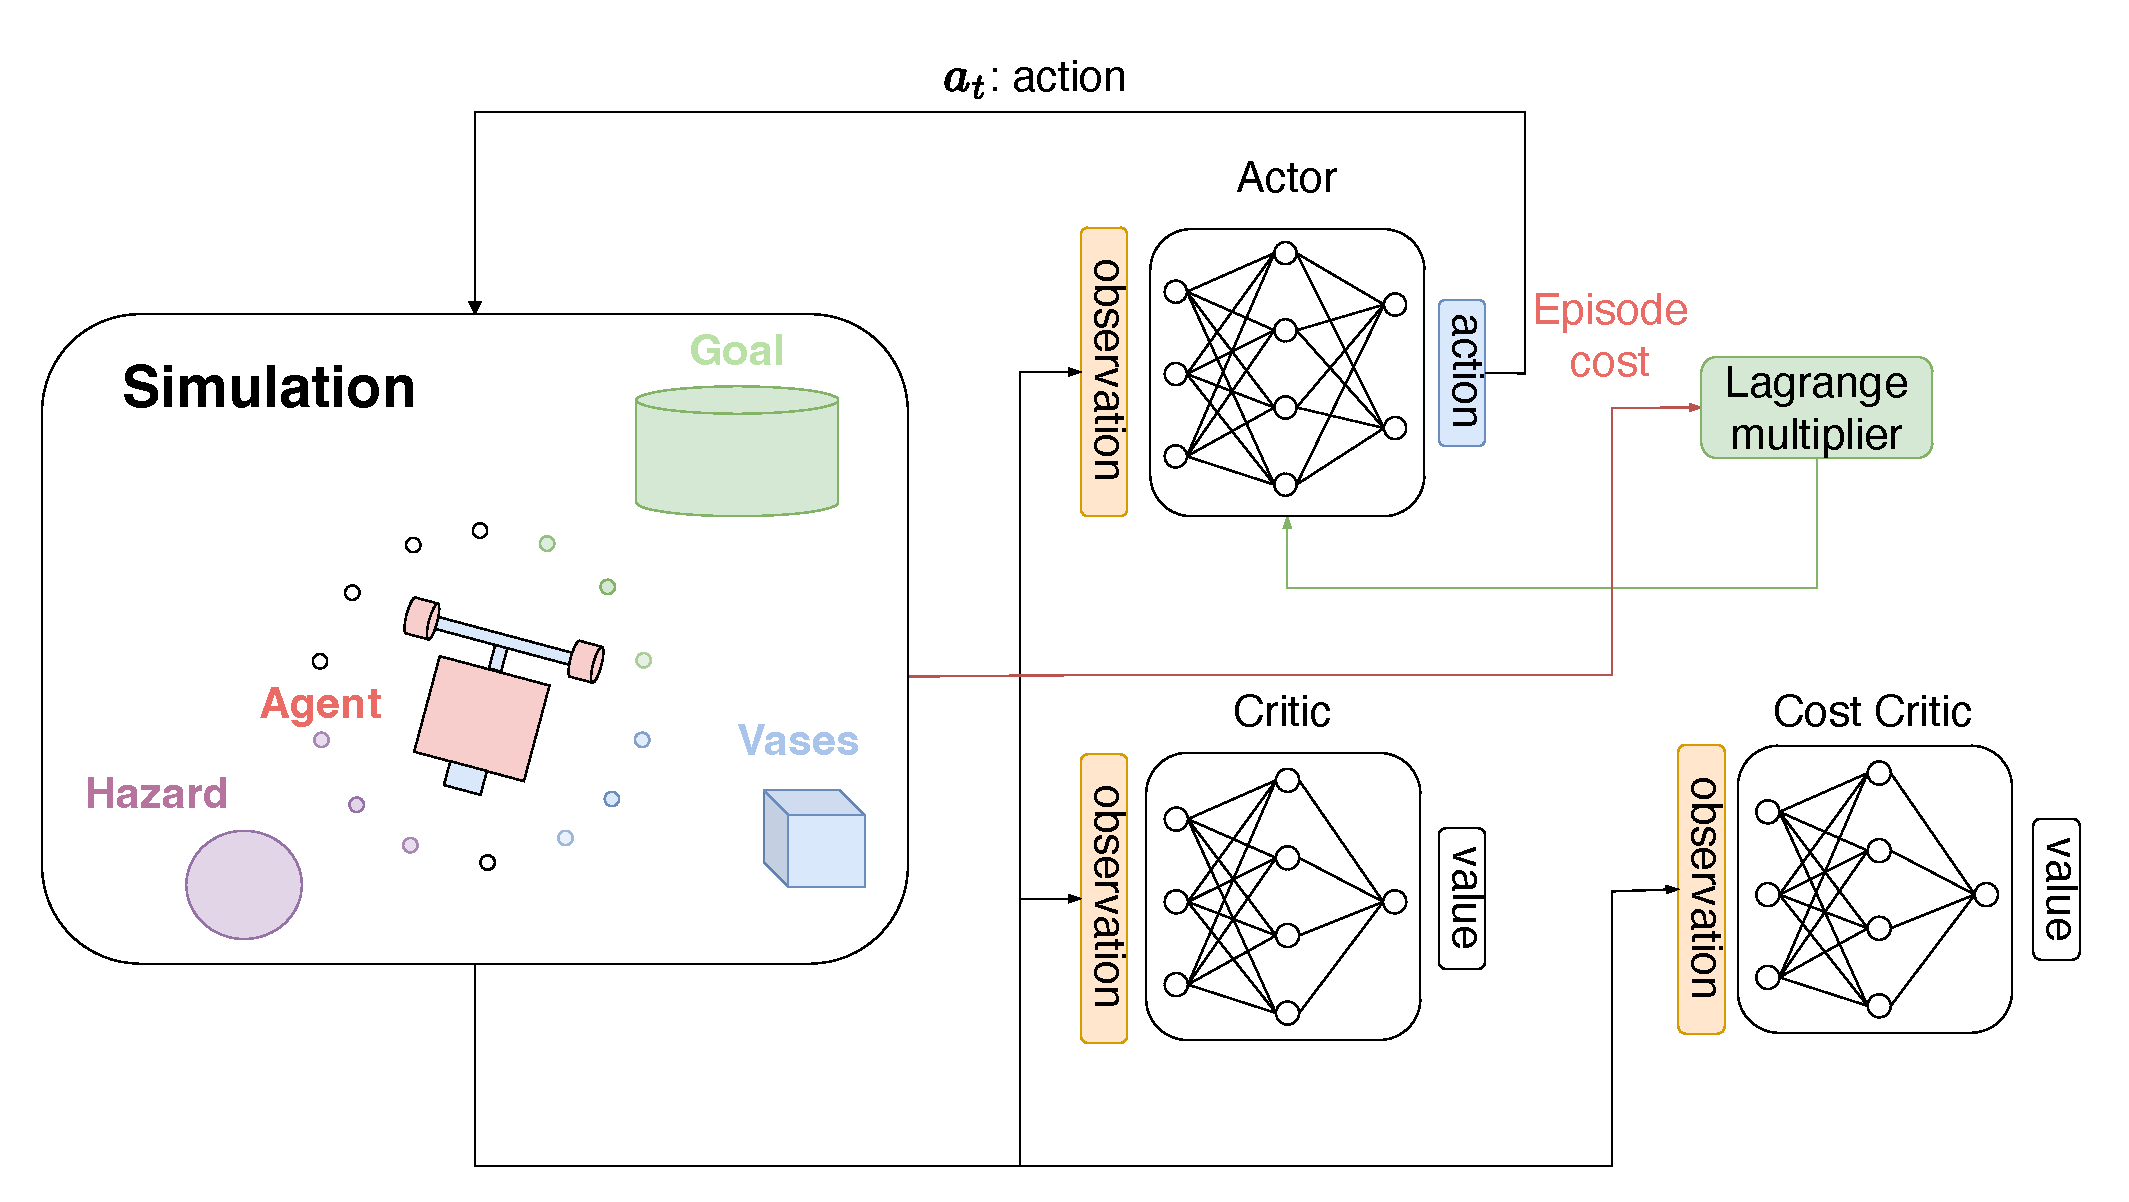
\includegraphics[width=1.0\textwidth]{imgs/chap2/ppo_lag.pdf}
  \caption{Structure of PPO Lagrangian}
  \label{chap2:fig:ppo_lag}
\end{figure*}

%%%%%%%%%%%%%%%%%%%%%%%%%%%%%%%%
\section{State-wise Constrained Reinforcement Learning} \label{chap2:sec5}
%%%%%%%%%%%%%%%%%%%%%%%%%%%%%%%%

State-wise Constrained Reinforcement Learning (SCRL) is a variant of CRL that imposes constraints at the state level.
CRL considers the cumulative cost over the entire trajectory, while SCRL focuses on the cost at each transition.
SCRL is formalized as a State-wise Constrained Markov Decision Process (SCMPD), it is quite similar to CMDP, but SCMDP enforces the constraint for every state action trasition satisfies a hard constraints.
The objective of SCRL is to find an optimal policy that maximizes the expected cumulative reward while satisfying the state-wise constraints.
\begin{equation}
  \begin{aligned}
    \pi^* &= \arg\max_{\pi_\theta} J(\theta) \\
    J(\theta) &= \mathbb{E}_{\tau \sim \pi_\theta} \left[ \sum^T_{t = 0} r_t \right] \; \text{subject to} \; \mathbb{E}_{\tau \sim \pi_\theta}  [c(s, a)] \leq w, \quad \forall s \in S
  \end{aligned}
\end{equation}

\subsection{Related Work: Feasible Actor-Critic} \label{chap2:sec5:fac}

Feasible Actor-Critic (FAC) is an extension of the Soft Actor-Critic algorithm to the SCRL setting \cite{FAC}.
In FAC, the state-wise constraint is enforced via a cost action-value function, formulated as:
\begin{equation}
  Q^{\pi_\theta}_c(s, a) = \mathbb{E}_{\tau \sim \pi_\theta}\left[\sum^T_{t = 0} c_t |s_0 = s, a_0 = ~a \right] \leq w
\end{equation}
The objective function of FAC is defined as:
\begin{equation} \label{chap2:eq:fac}
  \begin{aligned}
    J^{\text{FAC}}(\theta) = \mathbb{E}_{s_t \sim \mathcal{D}} \Big[ \mathbb{E}_{a_t \sim \pi_\theta} \big[ 
    &\alpha \log(\pi_\theta(a_t|s_t)) - Q_\phi(s_t, a_t) \\
    &+ \lambda_\xi(s_t)\left( Q_{\phi_c}(s_t, a_t) - w \right) 
    \big] \Big]
  \end{aligned}
\end{equation}
where $Q_{\phi_c}$ is the cost action-value function, and $\lambda_\xi$ is the Lagrange multiplier network, which estimate the Lagrange multiplier for each state.
The update of the Lagrange multiplier network depends on whether the cost action-value function exceeds the threshold $w$.
\begin{equation}
  J_\lambda(\xi) = \mathbb{E}_{s_t \sim \mathcal{D}} \left[ \mathbb{E}_{a_t \sim \pi_\theta} \left[ \lambda_\xi(s_t) \left( Q_{\phi_c}(s_t, a_t) - w \right) \right] \right]
\end{equation}
Fig.~\ref{chap2:fig:fac} illustrates the architecture of Feasible Actor-Critic (FAC). 
Since FAC is an off-policy algorithm, samples collected during the rollout phase are stored in a replay buffer, and mini-batches are drawn from it to update the actor, critics, and Lagrange multiplier network. 
The environment-provided reward and cost are used to update their respective Q-functions.
Using the reward and cost values estimated by the critic networks, together with the Lagrange multiplier computed from the Lagrange multiplier network, the policy is updated according to Equation~\ref{chap2:eq:fac}. 
The Lagrange multiplier network is updated based on the cost values estimated by the cost Q-function.
\begin{figure*}[h]
  \centering
  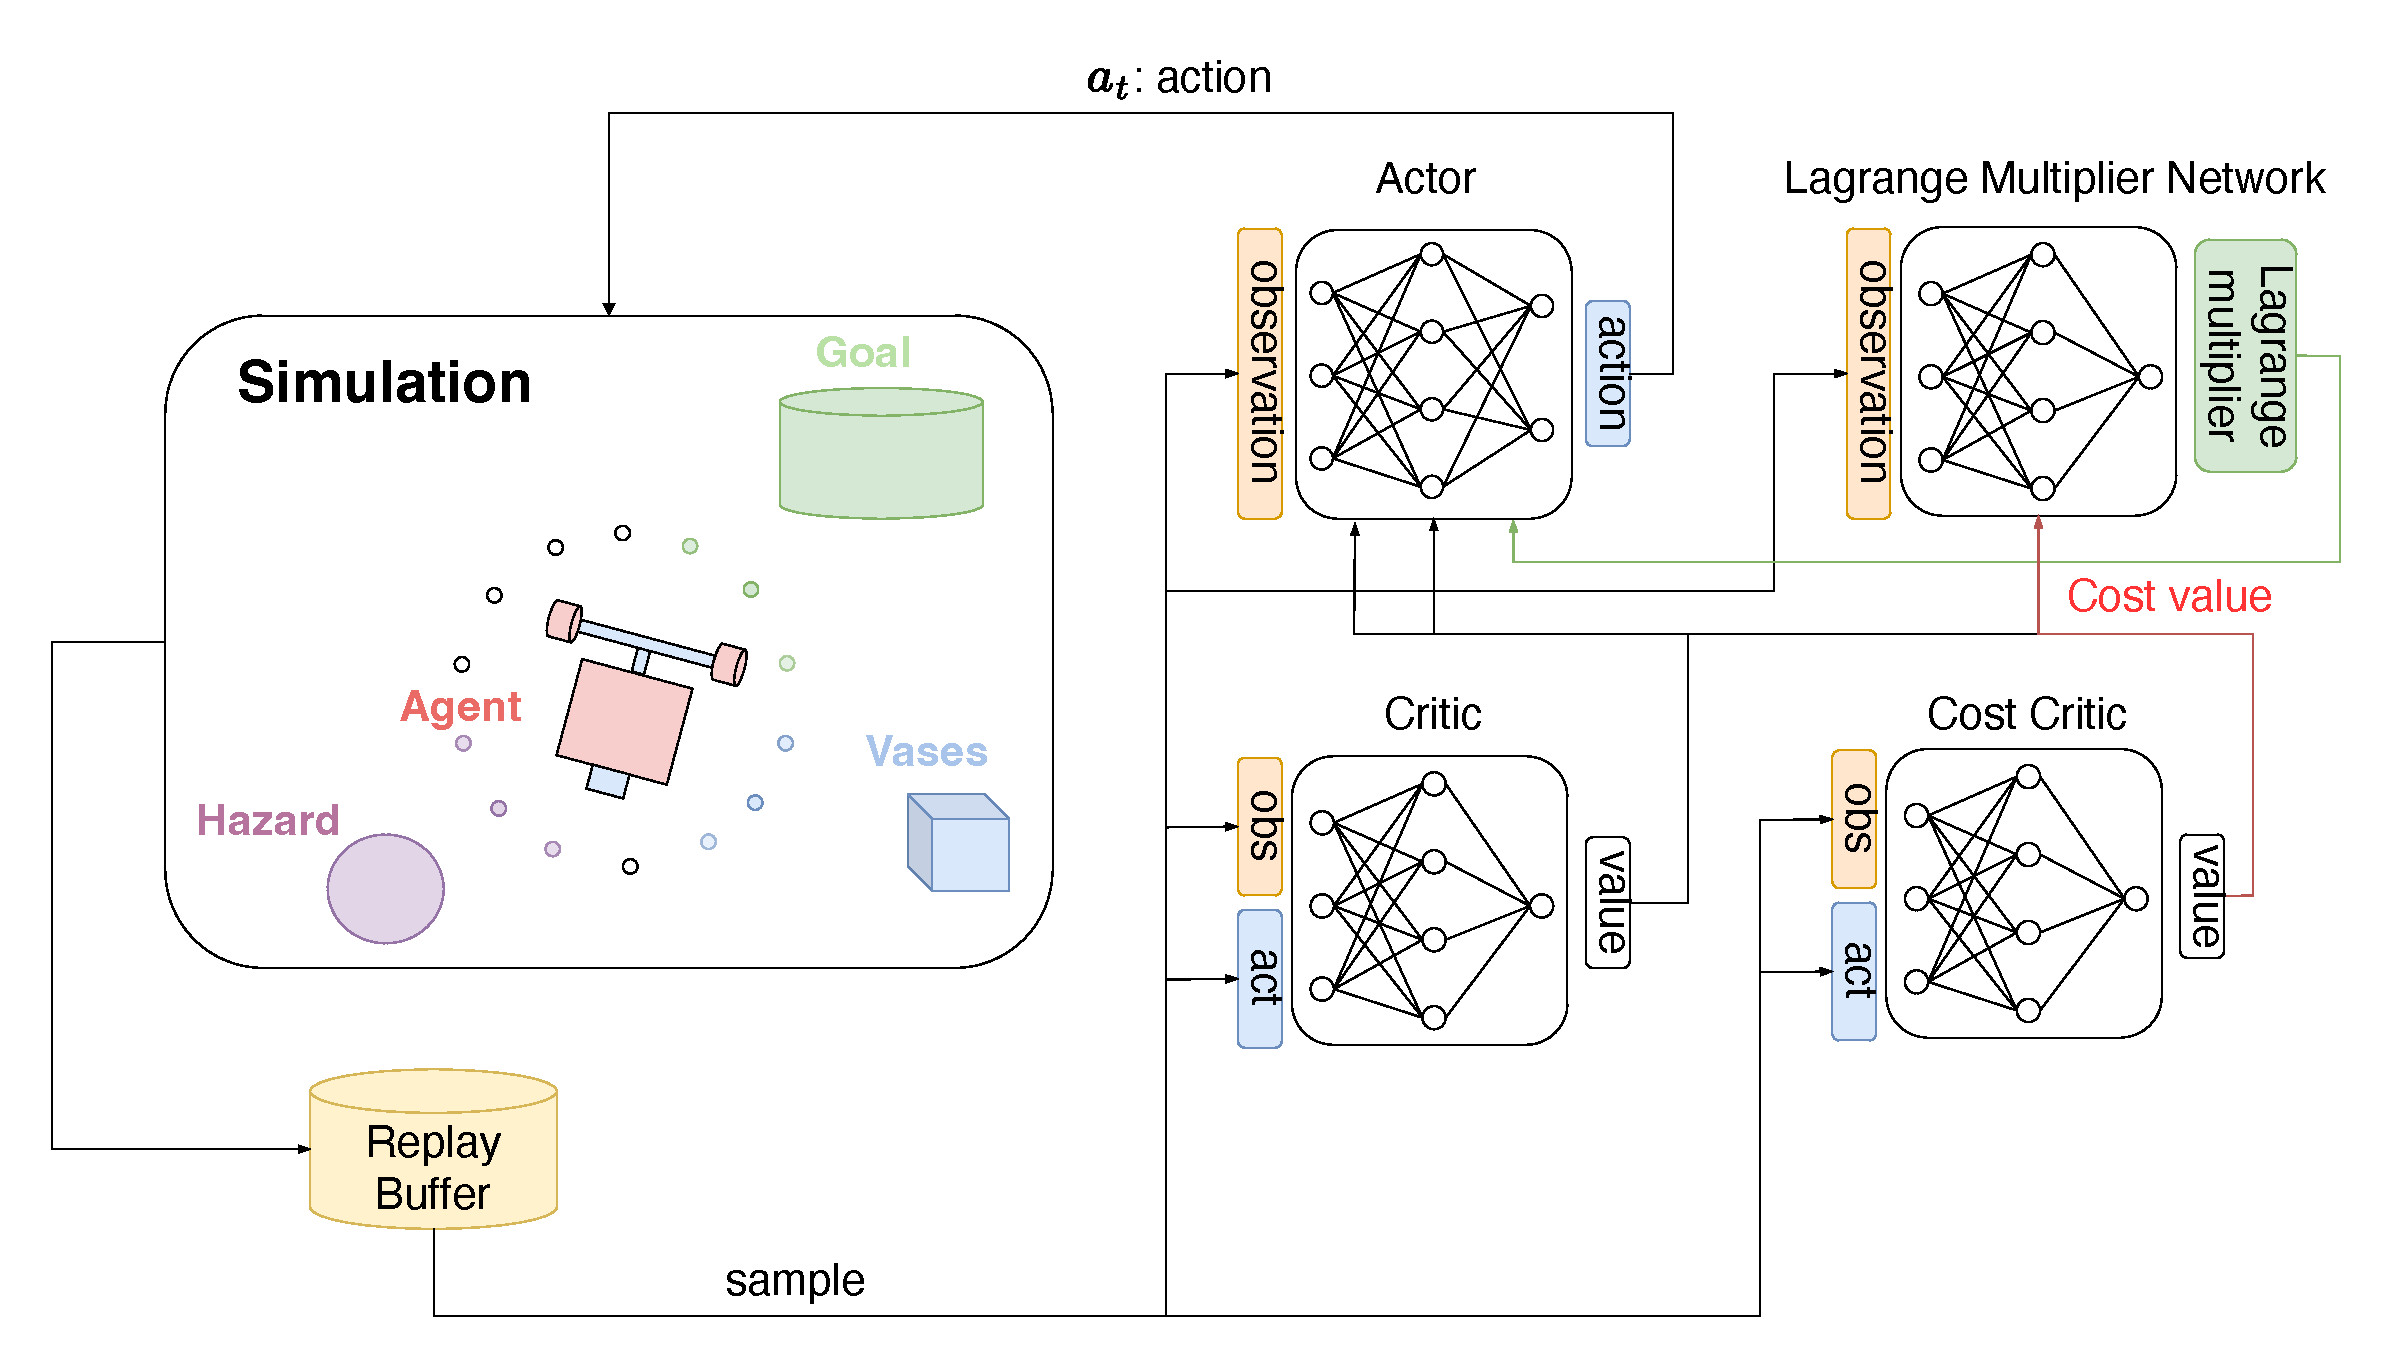
\includegraphics[width=1.0\textwidth]{imgs/chap2/fac.pdf}
  \caption{Structure of Feasible Actor-Critic}
  \label{chap2:fig:fac}
\end{figure*}

\noindent Although FAC contributes by proposing a framework that leverages a Lagrange multiplier network to address state-wise safety in policy learning, it has several limitations.
\begin{itemize}
  \item 
  Soft Actor-Critic (SAC) encourges exploration and promotes diverse action selection by adjusting the temperature parameter $\alpha$. 
  However, this objective can conflict with the constraint penalty term, which pushes the policy toward satisfying constraints. 
  As a result, it becomes more difficult for the policy consistently satisfy the constraints.
  \item 
  Instead of using the empirical cost values, FAC relies on a cost value estimated by the cost action-value function $Q_{\phi_c}(s, a)$.
  This introduces instability in the update of the Lagrange multiplier network due to potentially inaccurate cost estimates, which in turn can lead to unreliable policy updates.
\end{itemize}